\section{Chaos im Van der Pol System\label{vanderpol:section:chaos}}
\rhead{Chaos im Van der Pol System}

In die Gleichung \ref{vanderpol:equations:inhomogene_2} die Änderung der Amplitude $A$ verändert das Systemverhalten. Bei der Beobachtung der Frequenz des Oszillators wurden drei verschiedene Fälle erkannt. Wie in der Abb. \ref{vanderpol:figures:fft} gezeigt, ist die Frequenz des Van der Pol Oszillators dominant, wenn der Wert $A$ kleiner als der kritische Wert ist. Wenn der Wert höher ist, dominiert die Frequenz $\omega$. Beim kritischen Punkt gibt es eine Summe von Frequenzen im System. Durch Setzen der Werte $\mu=0.2$ und $\omega=1.15$ beträgt der kritische Wert von $A$ in diesem Fall $0.32$. Wie in die Gleichung
\begin{equation}
	\ddot{x}-0.2\left(1-x^{2}\right) \dot{x}+x = A \cdot \sin(1.15 t).
	\label{vanderpol:equations:inhomogene_3}
\end{equation}

\begin{figure}
	\centering
	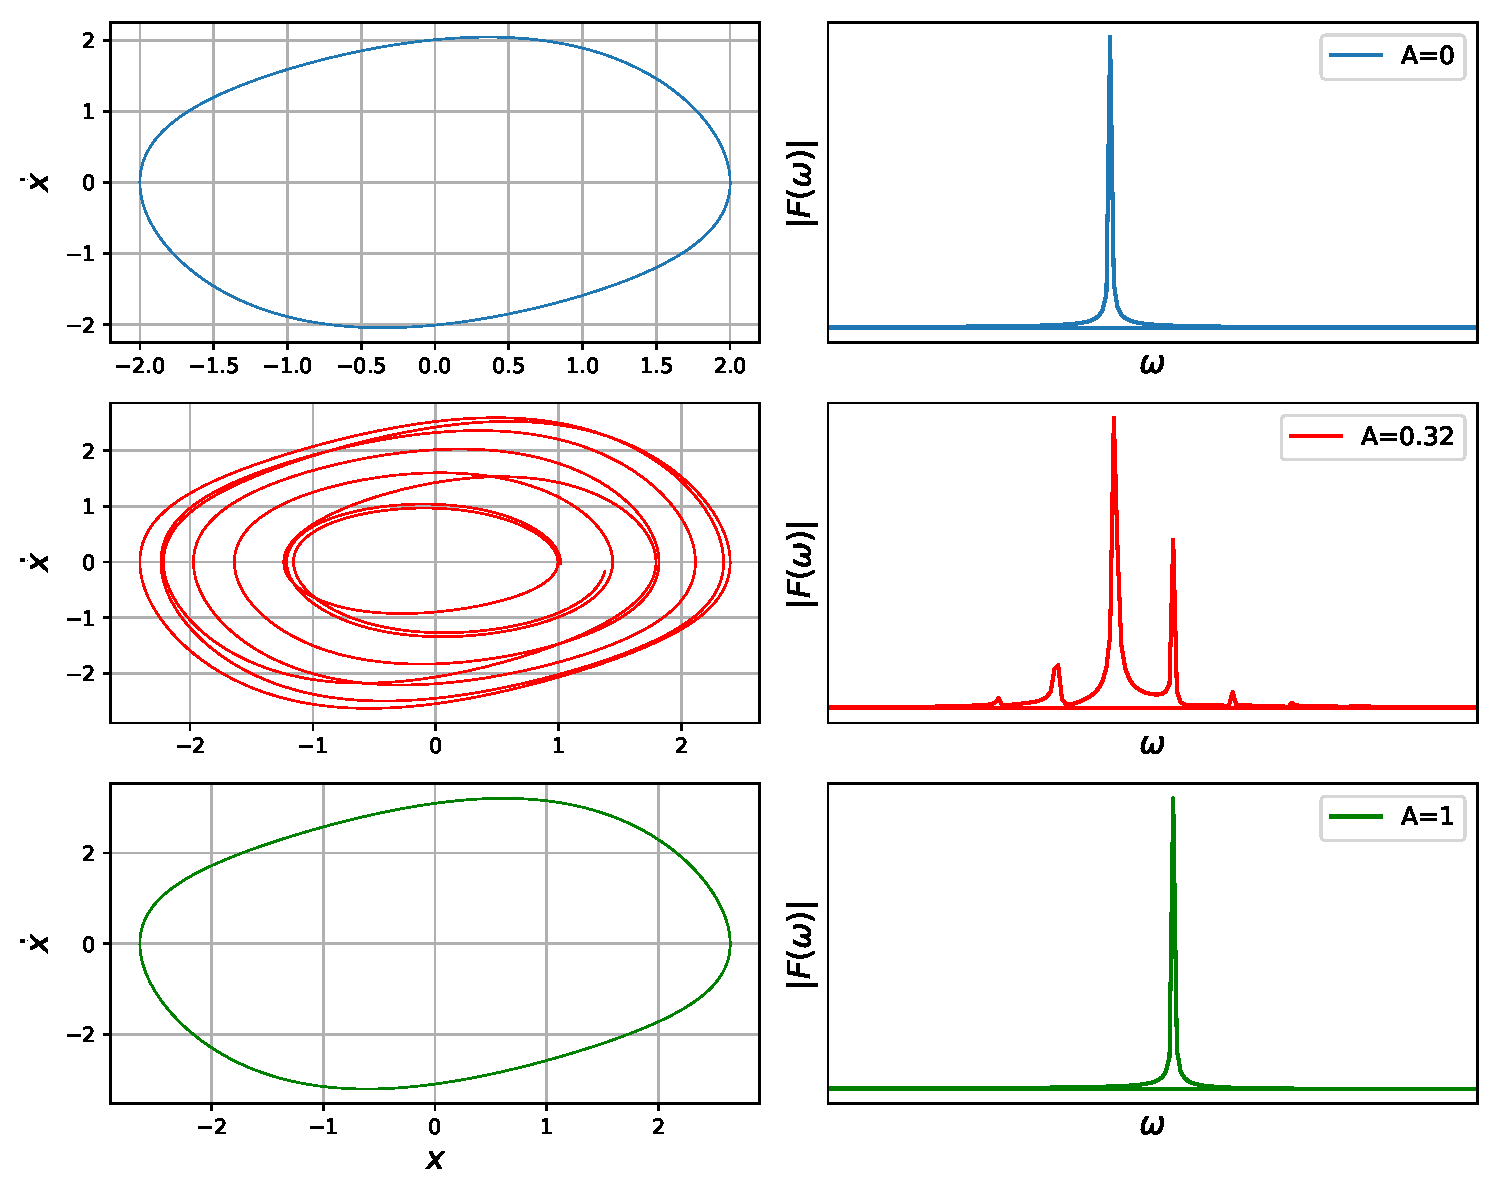
\includegraphics[width=0.9\textwidth]{papers/vanderpol/figures/fft_plot2.pdf}
	\caption{Phaseraum Diagramm und Frequenzspektrum der Gleichung \ref{vanderpol:equations:inhomogene_3} mit verschiedenen Werten von $A$.\label{vanderpol:figures:fft}}
\end{figure}

\subsection{Anfangsbedingung}
\label{vanderpol:subsection:anfangsbedingung}
\begin{cquote}[30pt]{Edward Lorenz}
``Chaos: When the present determines the future, but the approximate present does not approximately determine the future.''
\end{cquote}
\noindent Das angeführte Zitat ist genau die Definition, die das in diesem Kapitel untersuchte Problem erklärt, nämlich die Instabilität der numerischen Methoden. Letztere führen zu einem Rundungsfehler, der sich während der verschiedenen Iterationen ansammelt. Diese hängt von der für den Integrationsschritt gewählten Länge ab. Mehrere Längen entsprechen daher unterschiedlichen Werten des Fehlers. Per Definition ist ein chaotisches System sehr empfindlich gegenüber Veränderungen, auch wenn diese minimal sind. Zwei Fehler aufgrund von zwei unterschiedlichen Integrationsschritten können somit zu zwei völlig unterschiedlichen Lösungen führen. In der Regel tritt die Divergenz zwischen den beiden Lösungen nach einer bestimmten Zeitspanne auf. Etwas Ähnliches geschieht, wenn, immer in einem chaotischen System, eine kleine Variation der Anfangsbedingungen eingeführt wird. Dieser kleine Unterschied kann, analog zu dem durch Fehler verursachten, das Langzeitverhalten des Systems stark beeinflussen. Diese Empfindlichkeit gegenüber Veränderungen im Ausgangszustand ist auch bekannt als {\em Butterfly Effect}. Zur Erklärung dieses Phänomens verwendete Edward Lorentz in 1972 auf einer Konferenz diesen Satz:``Ein Schmetterling schlägt in Peking mit den Flügeln, und in New York kommt Regen statt Sonne''.
\begin{figure}
\centering
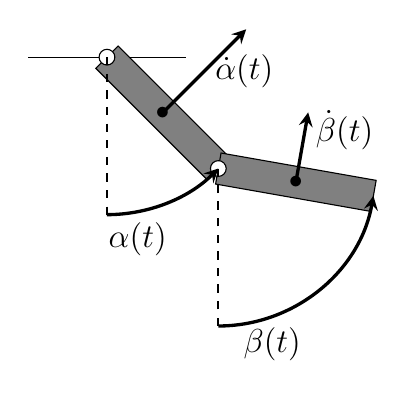
\begin{tikzpicture}[scale=1]

\draw (-1,0) -- (1,0);

\begin{scope}[rotate=45]

\draw[fill=gray]  (-0.2, 0) rectangle (0.2,-2.0) node[midway](a){$\bullet$};
%alpha'(t)
\draw[->, very thick, -stealth](0.0,-1.0) -- (1.5, -1.0) node[midway, right]{\large $\dot{\alpha}(t)$};

\draw[fill=gray, rotate around={35:(0, -2.0)}] (-0.2,-2.0) rectangle (0.2,-4.0)node[midway](a){$\bullet$};
%beta'(t)
\draw[->,very thick, -stealth, rotate around={35:(0, -2.0)}](0,-3.0) -- (0.9, -3.0) node[near end, above, right]{\large $\dot{\beta}(t)$};

\draw[fill=white] (0,-2.0) circle(0.1);
\draw[fill=white] (0,0) circle(0.1);

\end{scope}

\draw[very thick, ->, -stealth](0,-2.0) arc (-90:-45:2) node[near start, below]{\large $\alpha(t)$};
\draw[thick,dash pattern=on 3 off 3] (0,0) -- (0,-2.0);

\draw[very thick, ->, -stealth](1.414,-3.414) arc (-90:-10:2) node[near start, below]{\large $\beta(t)$};
\draw[thick,dash pattern=on 3 off 3] (1.414,-3.414)--(1.414,-1.414);

\end{tikzpicture}
\caption{Doppelpendel\label{vanderpol:figures:doublependulum}}
\end{figure}
Kann also eine solch minimale Veränderung der Anfangsbedingungen das Endergebnis vollständig verändern? Die Antwort ist offensichtlich ja, was auch durch die Grafiken auf den folgenden Seiten bewiesen wird.
\subsubsection{Doppelpendel}
\label{vanderpol:subsubsection:doppelpendel}
Im Falle des Bildes Abb. \ref{vanderpol:figures:init_cond_dbl_pend} wurde die Lösung des im Abb. \ref{vanderpol:figures:doublependulum} dargestellten Systems, ein Doppelpendel, berichtet. Es wird natürlich nicht im Detail behandelt, da dies nicht die Aufgabe dieses Kapitels ist. Es handelt sich jedoch um ein praktisches Beispiel, das genau zeigt, was im Anfangszitat zusammengefasst ist. Die beiden gezeigten Funktionen stellen den $\alpha$ Winkel zweier Doppelpendel mit Anfangsbedingungen dar, die eine geringe Abweichung aufweisen. Die Ausgangssituation wird also durch die folgenden Werte beschrieben:

\begin{itemize}
\item
$\alpha_1(0) = \frac{\pi}{2}$
\item
$\alpha_2(0) = \alpha_1(0) + \delta, \quad \delta = 10^{-3}$
\item
$\dot{\alpha_1}(0) = \dot{\alpha_2}(0)= 1 \frac{m}{s}, \quad \dot{\beta_1}(0) = \dot{\beta_2}(0)= 1 \frac{m}{s}, \quad \beta_1(0)=\beta_2(0)=\frac{\pi}{2}$
\end{itemize}

\begin{figure}
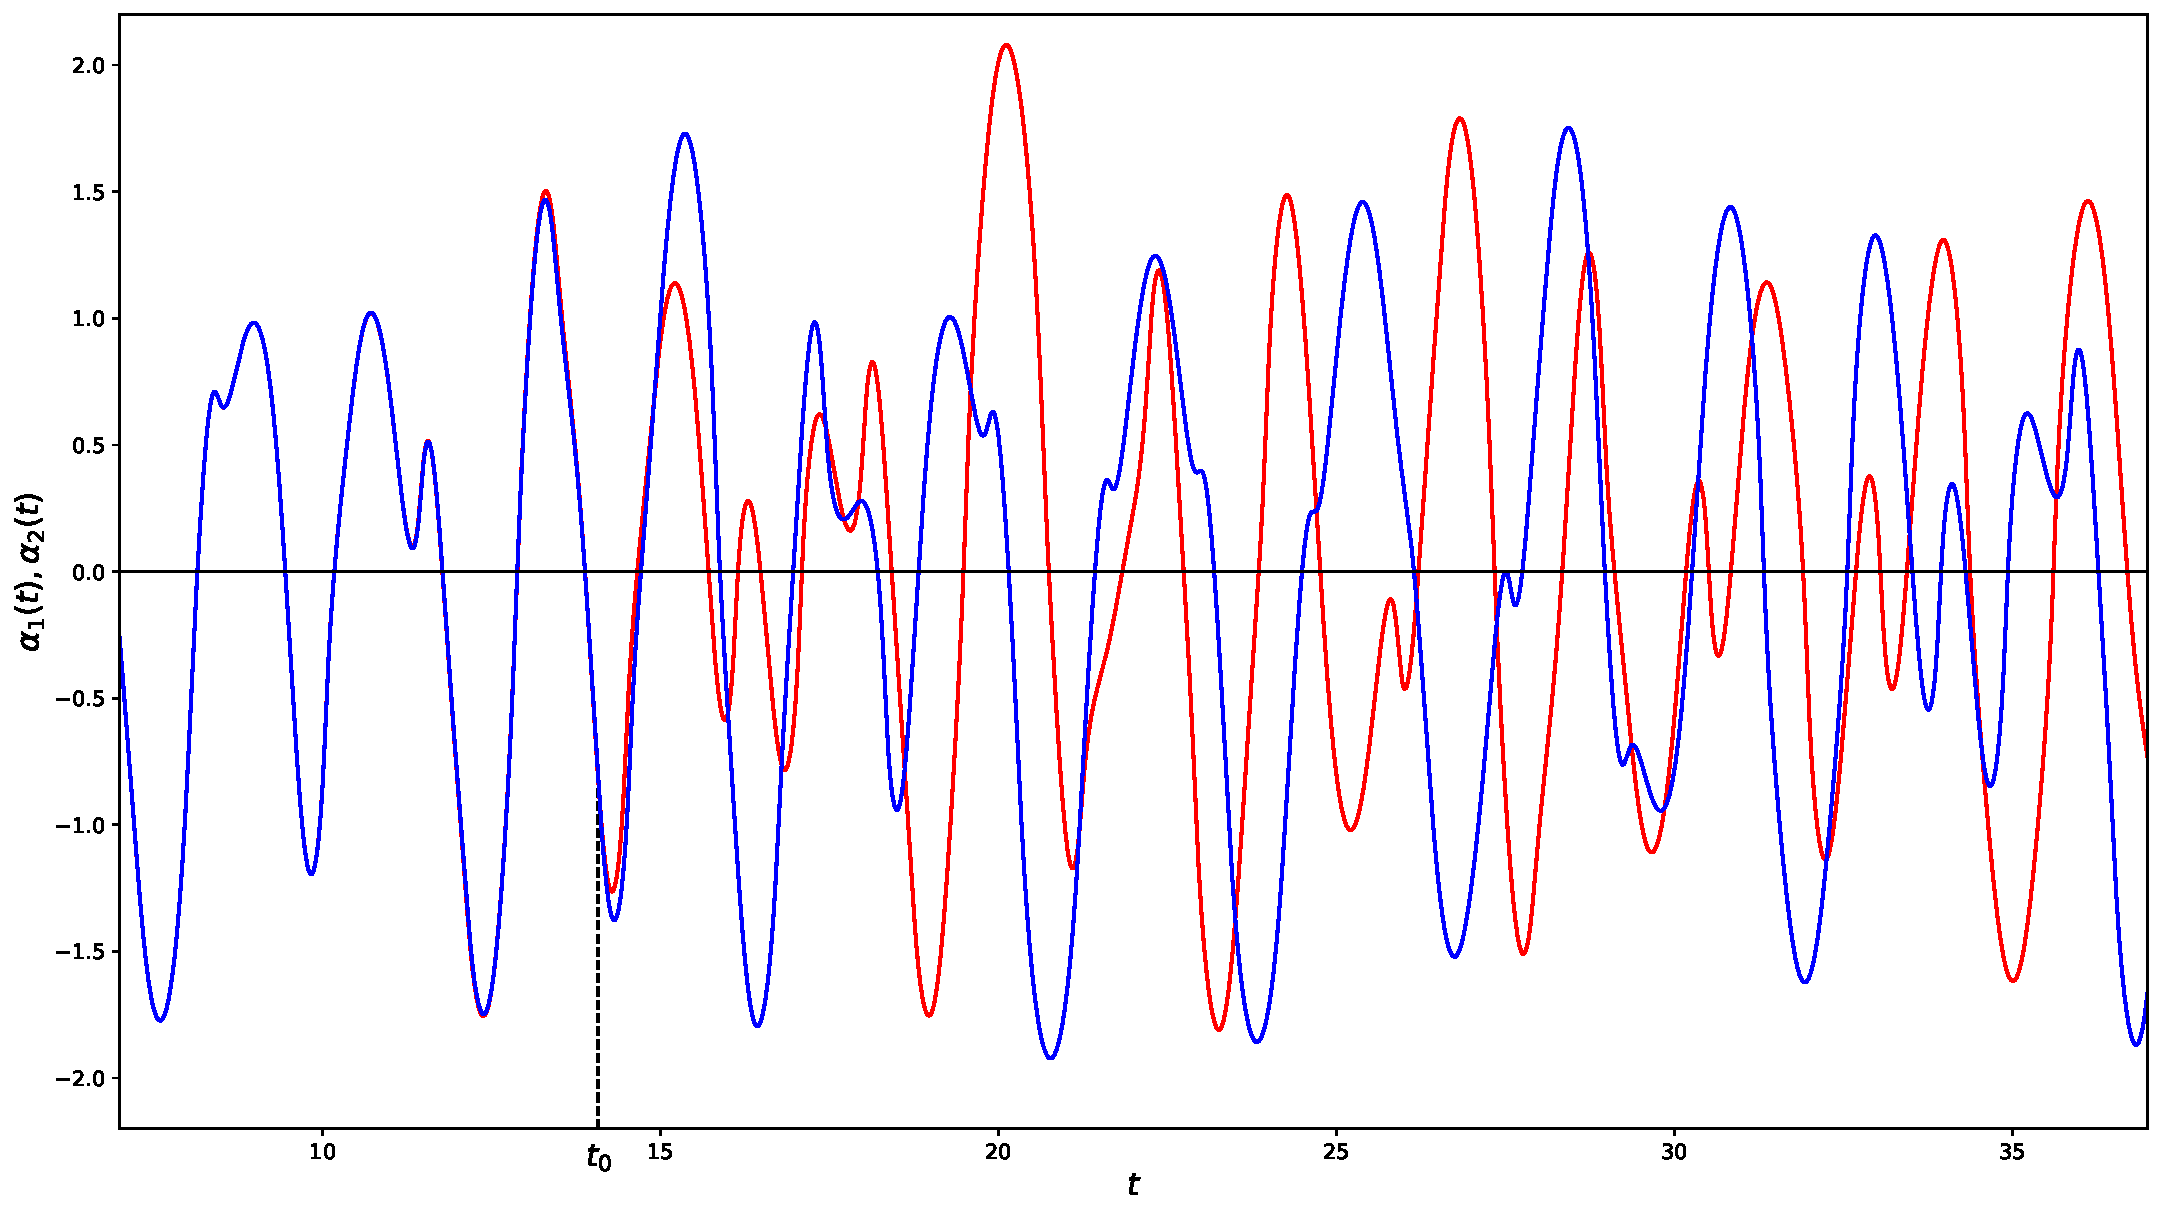
\includegraphics[width=\textwidth]{papers/vanderpol/figures/initial_cond_DBLPEND.pdf}
\caption{Verlauf der Winkel $\alpha_1(t)$, $\alpha_2(t)$ des Doppelpendels in Abb. \ref{vanderpol:figures:doublependulum} und Angabe des Divergenzpunktes $t_0$\label{vanderpol:figures:init_cond_dbl_pend}}
\end{figure}
\noindent Wie in Abb. \ref{vanderpol:figures:init_cond_dbl_pend} zu sehen ist, überlagern sich die beiden Lösungen im Anfangsmoment und sind nicht zu unterscheiden. Ab dem Punkt $t_0$ merkt man, dass sie plötzlich ganz andere Bahnen verfolgen. Die geringe anfängliche Varianz von $\delta$ hat daher die Endergebnisse in nicht gleichgültiger Weise beeinflusst.
\subsubsection{Van der Pol Gleichung}
\label{vanderpol:subsubsection:vdp}
Dasselbe geschieht auch im Fall der Van der Pol Gleichung. Im  Abb. \ref{vanderpol:figures:init_cond_VDP} sind zwei Darstellungen des Verlaufs der beiden mit dem gleichen Integrationsschritt erhaltenen numerischen Lösungen der Gl. \ref{vanderpol:equations:inhomogene_2} im Zeitbereich gezeigt. Die Anfangsbedingung sind in diesem Fall wie folgt gewählt worden:

\begin{figure}
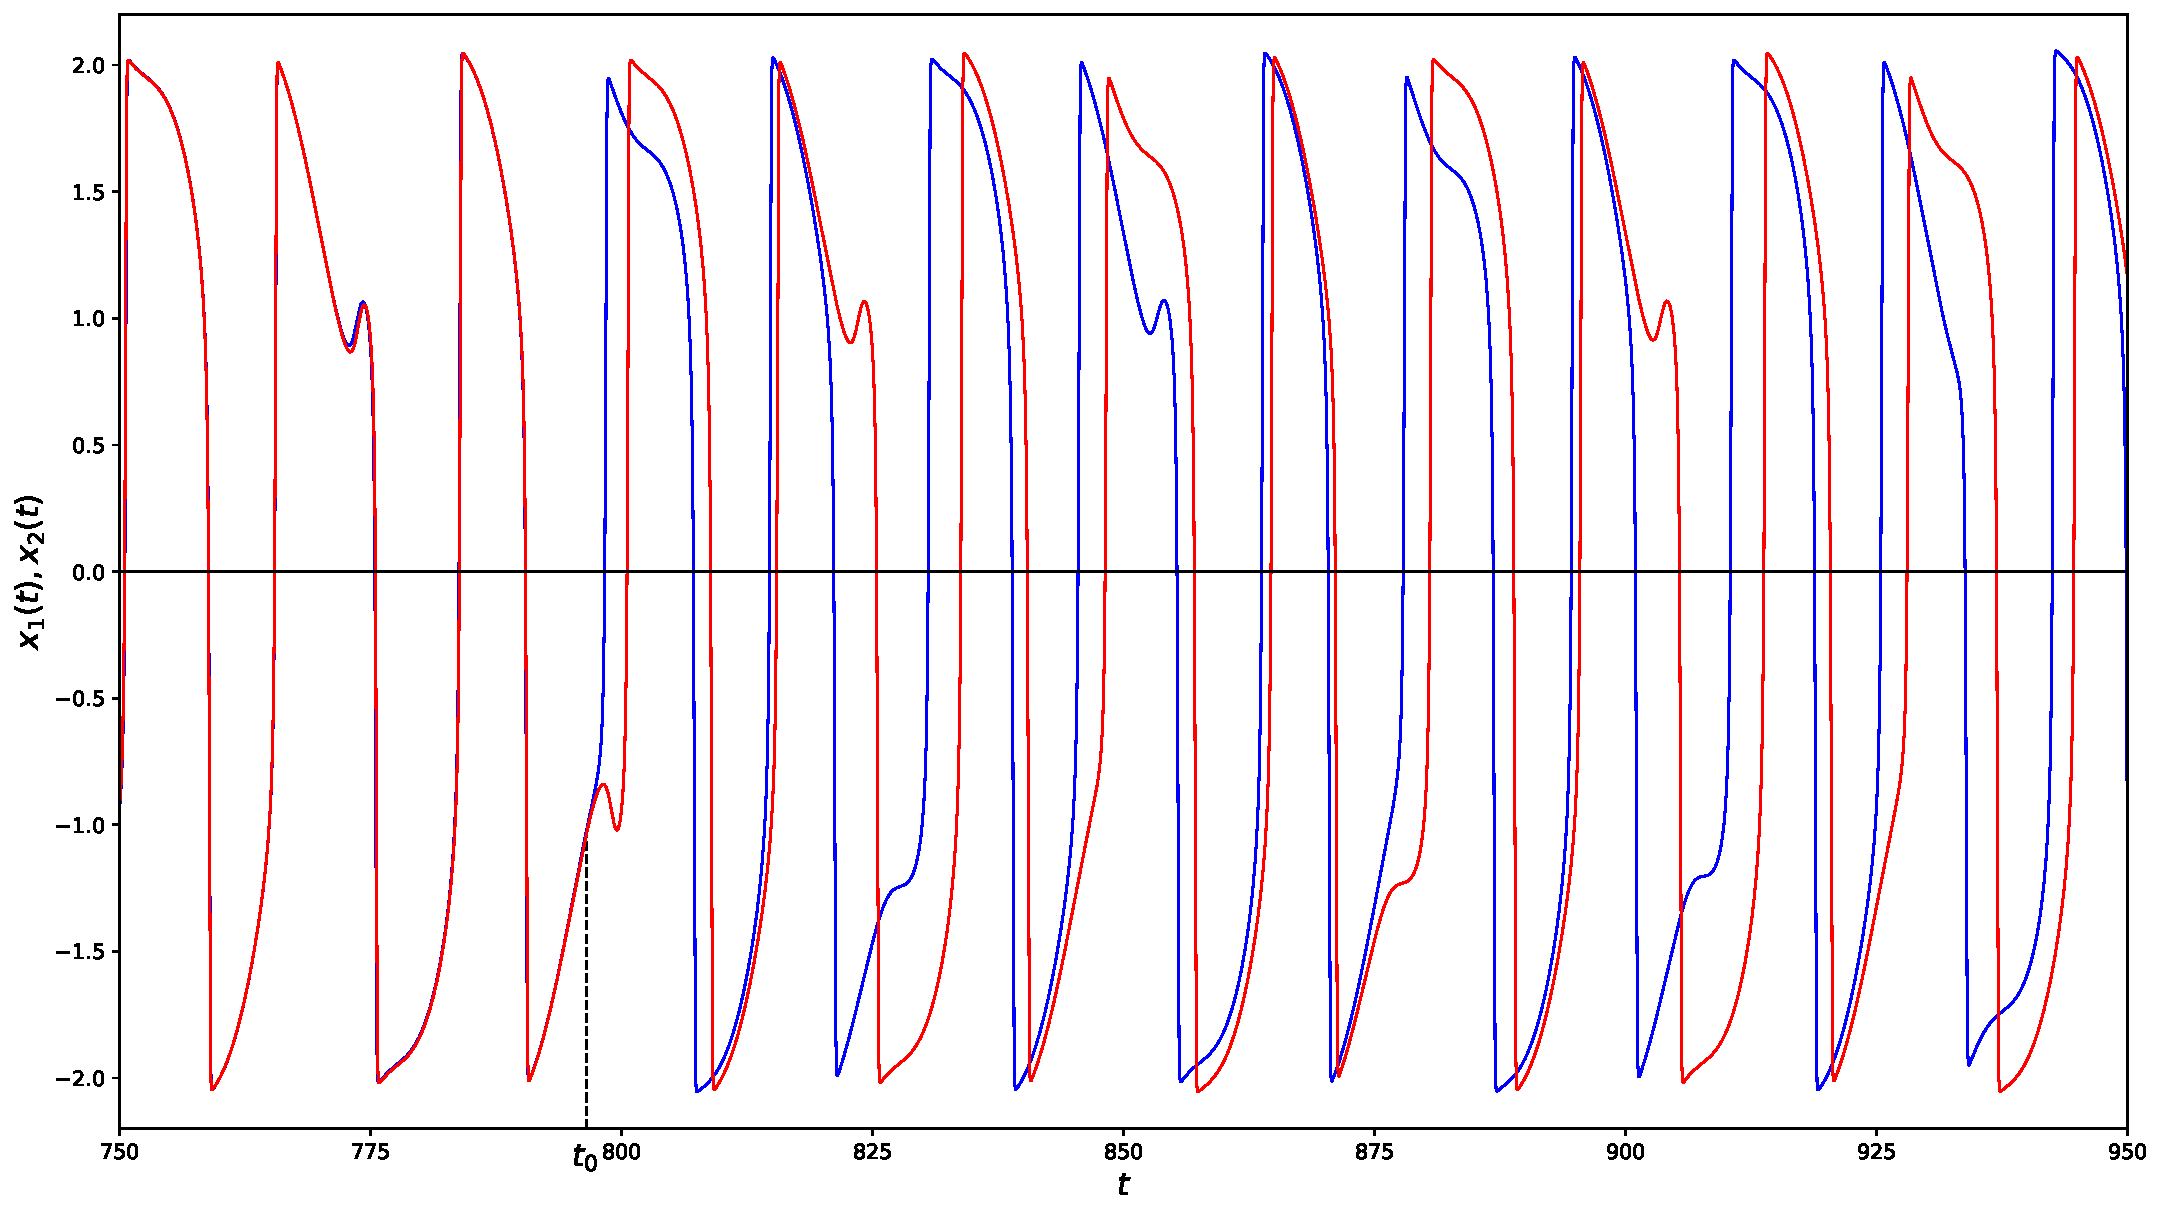
\includegraphics[width=\textwidth]{papers/vanderpol/figures/initial_cond_VDP.pdf}
\caption{Verlauf der Lösungen $x_1(t)$, $x_2(t)$ der Gl. \ref{vanderpol:equations:inhomogene_2} und Angabe des Divergenzpunktes $t_0$ \label{vanderpol:figures:init_cond_VDP}}
\end{figure}

\begin{itemize}
\item
$\dot{x_1}(0) = 5$
\item
$\dot{x_2}(0) = \dot{x_1}(0) + \delta, \quad \delta = 10^{-3}$ 
\item
$x_1(0) = x_2(0) = 0$
\end{itemize}
Daraus lässt sich natürlich schliessen, dass beide Systeme aufgrund ihrer chaotischen Natur sehr empfindlich auf die Anfangsbedingungen reagieren. Dies lässt sich auf den Zitat zurückführen, denn im Falle einer numerischen, nämlich eine approximativen Lösung $\hat{y}$, gilt dass

\begin{equation} 
|\hat{y}(x_n) - y(x_n)| = \epsilon.
\end{equation}
Obwohl $\epsilon$ ein sehr kleiner Wert sein kann, kann er unter bestimmten Umständen die gleiche Wirkung haben wie eine Änderung der Anfangsbedingungen. Dank der beiden Diagramme Abb.   \ref{vanderpol:figures:init_cond_VDP} und Abb. \ref{vanderpol:figures:init_cond_dbl_pend} konnte man feststellen, dass der Unterschied zwar in der Grössenordnung von $10^{-3}$ lag, aber nach einiger Zeit zu einer völlig anderen Topologie führte. Wie im nächsten Kapitel erläutert, gilt dies auch für die Änderung des Integrationsschrittes.

\subsection{Ergebnisse
\label{vanderpol:section:ergebnisse}}
Nachstehend sind die Ergebnisse der beiden oben beschriebenen Algorithmen aufgeführt. Die ausgewählten Anfangsbedingungen sind:
\begin{itemize}
\item
$\dot{x_1}(0) = \dot{x_2}(0) = 5$
\item
$x_1(0) = x_2(0) = 0$
\end{itemize}
In diesem Fall wurden im Gegensatz zu den in Abb.\ref{vanderpol:figures:init_cond_VDP} gezeigten Daten zwei verschiedene Integrationsschritte gewählt. Die Ergebnisse sind jedoch fast die gleichen. Im Falle der Runge Kutta Lösung wird deutlich, dass der Divergenzpunkt aufgrund der Änderung der Integrationsschritt noch vor dem liegt, der sich durch die Veränderung der Anfangsbedingungen ergibt. Auch in diesem Fall verursachte eine Differenz in der Grössenordnung von $10^{-3}$ eine starke Abweichung. Der Runge Kutta Algorithmus hat einen Rundungsfehler in der Grössenordnung von $O(h^5)$, während Euler $O(h^2)$ hat. Dies wirkt sich auf die Zeit $t_0$ aus, wenn Chaos eintritt. Im ersten Fall haben wir $t_0 \cong 770,5$ wie in Abb. \ref{vanderpol:figures:RK_schritt_e-3} gezeigt, während im zweiten Fall $t_0 \cong 59,7$ wie in Abb. \ref{vanderpol:figures:EULER_schritt} gezeigt.
In den folgenden Plots wird gezeigt, wie die Abnahme des Integrationsschrittes $h$ immer zu einem Divergenzpunkt $t_0$ führt, an dem das System chaotisch wird. Im Fall von Abb. \ref{vanderpol:figures:RK_schritt_2e-3} ist der Schritt $h_1=0.007$ und $h_2=0.009$ . In Abb. \ref{vanderpol:figures:RK_schritt_2e-3_2} wird die Schrittlänge auf $h_1=0.005$ und $h_2=0.007$ verringert. 

\begin{figure}
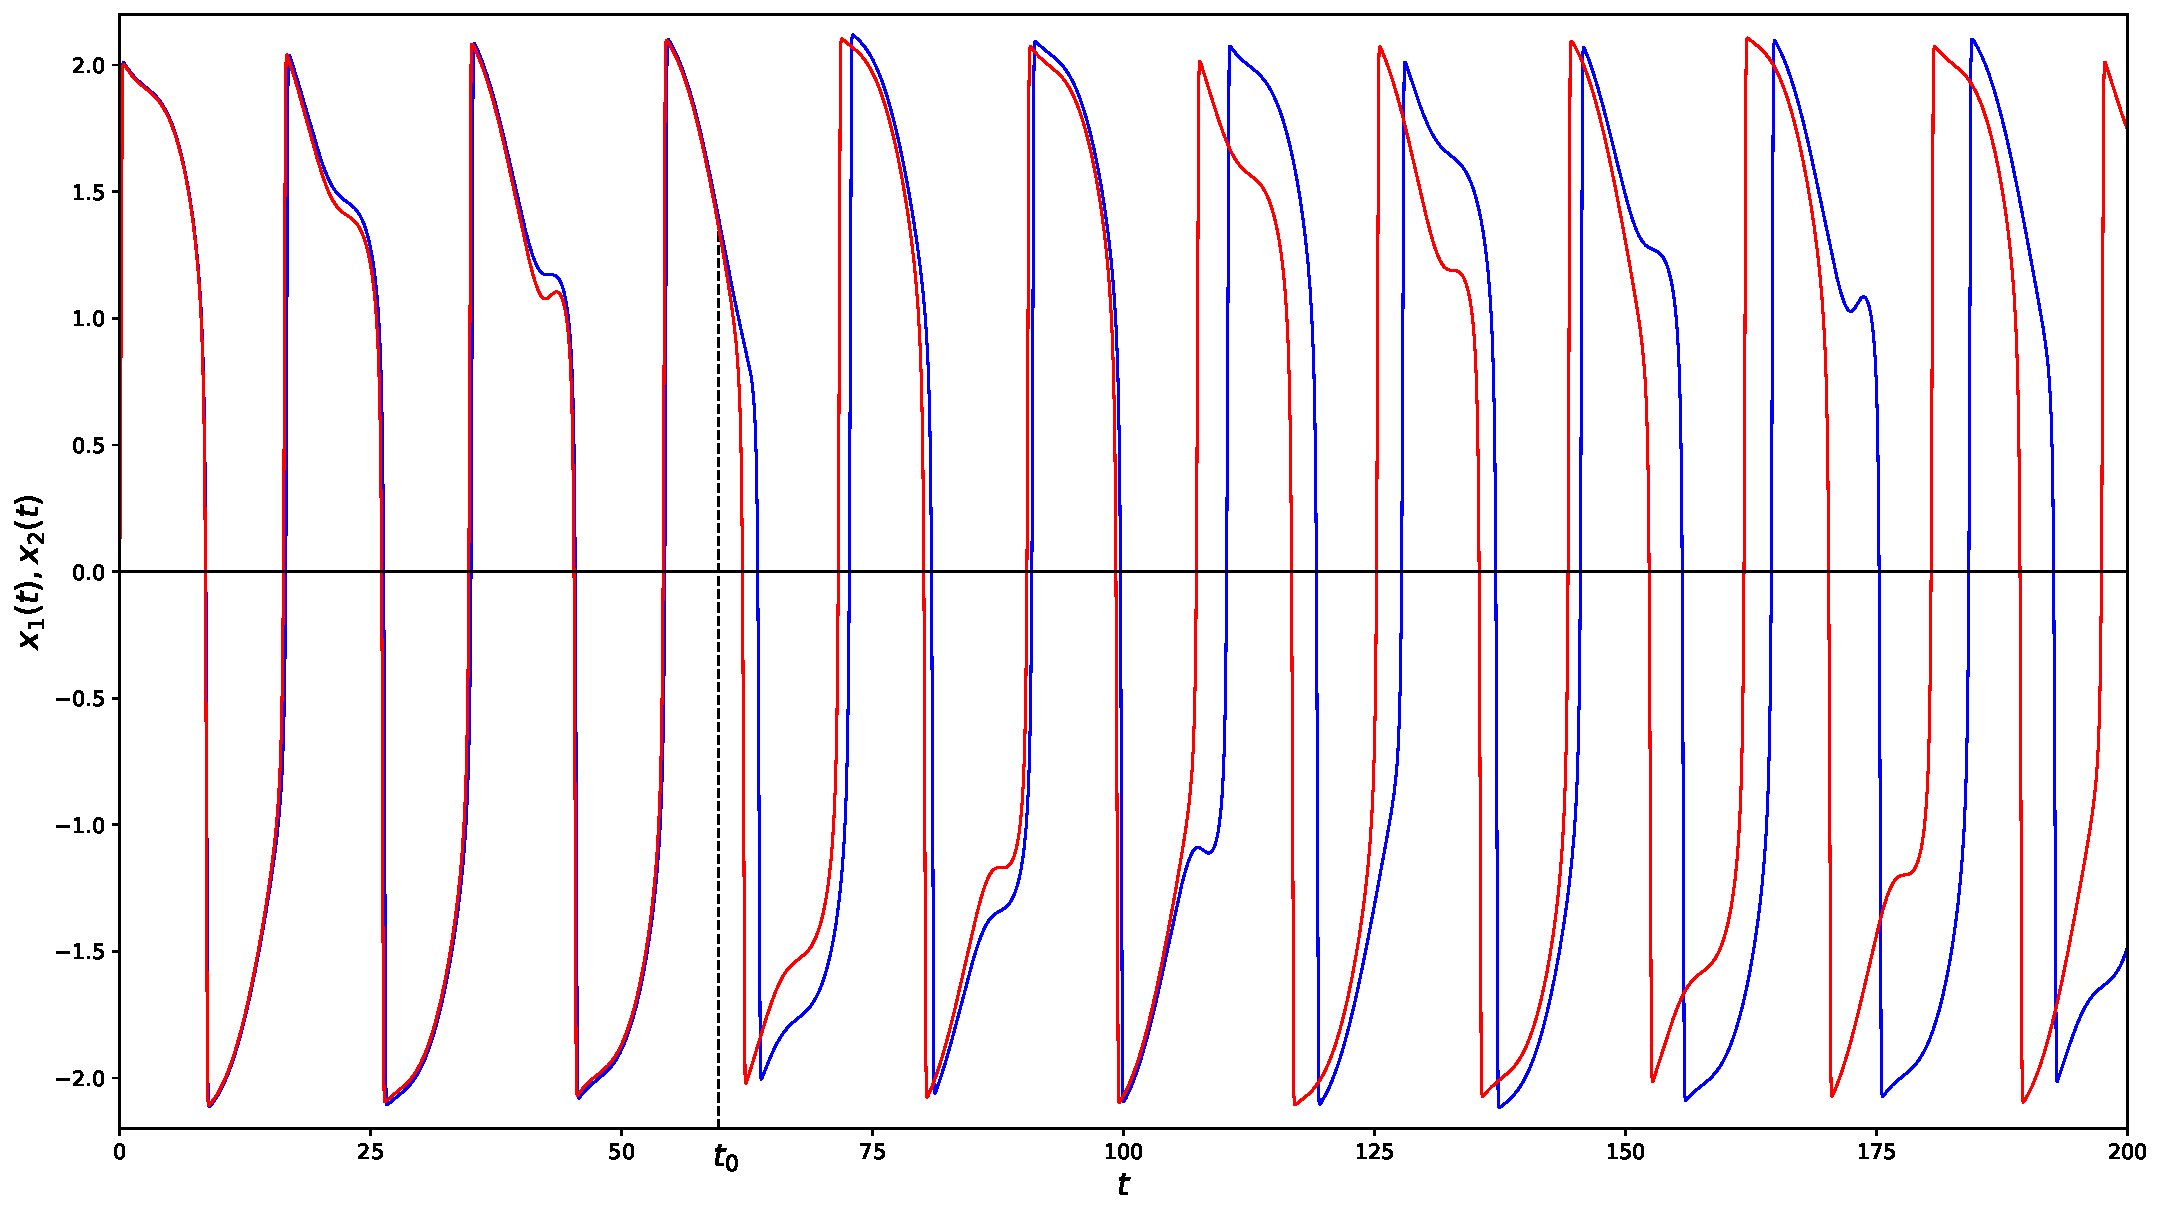
\includegraphics[width=\textwidth]{papers/vanderpol/figures/EULER_schritt_delta_e-3.pdf}
\caption{Verlauf der beiden mit der {\em Euler Methode} berechneten Lösungen $x_1$ und $x_2$ der Gl. \ref{vanderpol:equations:inhomogene_2} im Zeitbereich und Angabe des Divergenzpunktes $t_0$. Integrationsschritte: $h_1 = 0.01, \quad h_2 = 0.009$\label{vanderpol:figures:EULER_schritt}}
\end{figure}

\begin{figure}
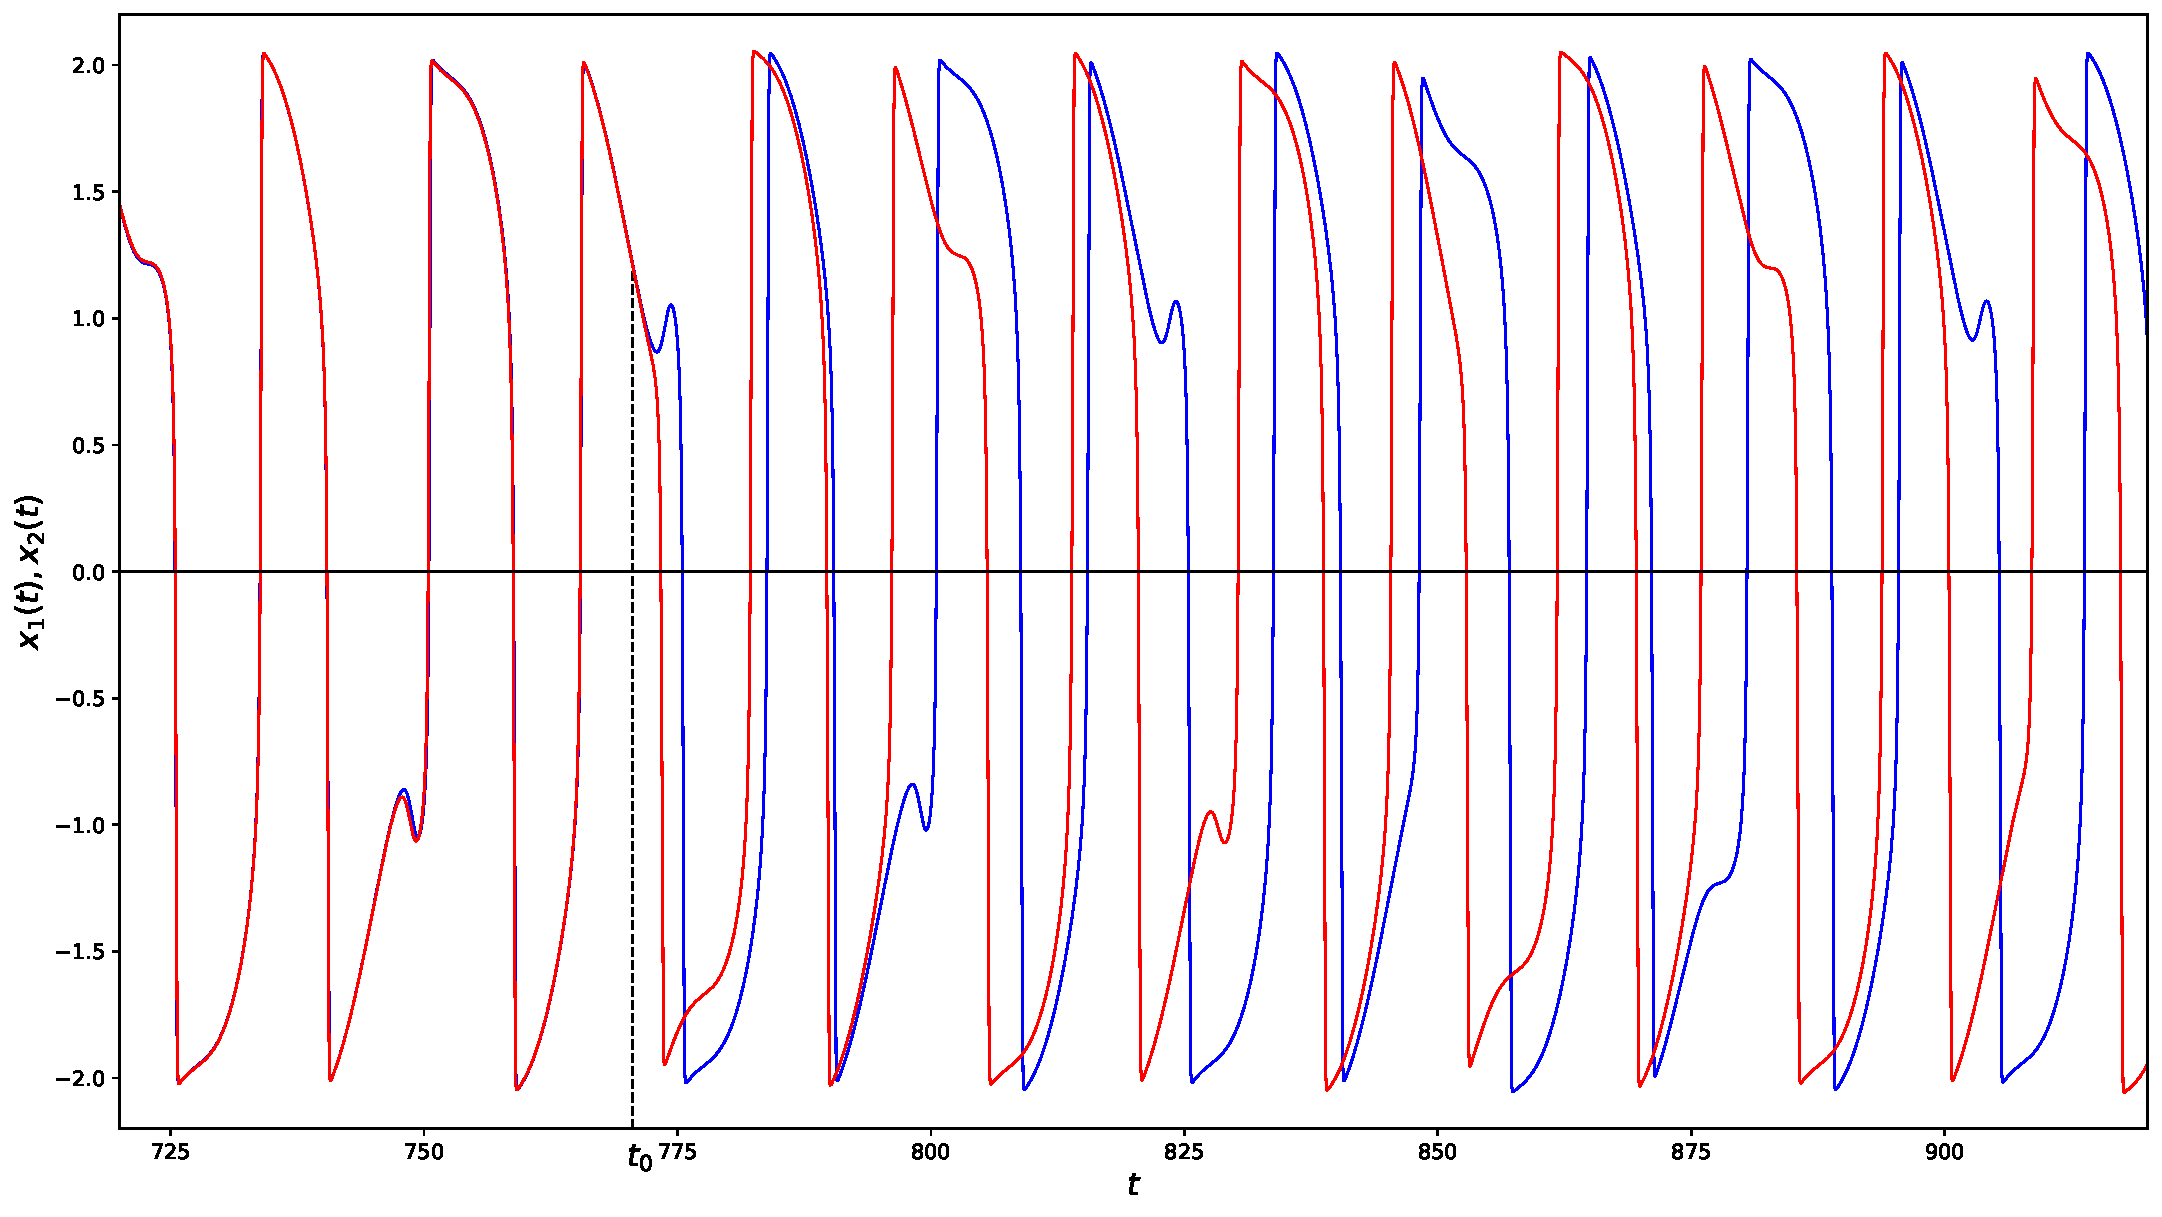
\includegraphics[width=\textwidth]{papers/vanderpol/figures/RK_schritt_delta_e-3.pdf}
\caption{Verlauf der beiden mit der {\em Runge Kutta Methode vierter Ordnung} berechneten Lösungen $x_1$ und $x_2$ der Gl. \ref{vanderpol:equations:inhomogene_2} im Zeitbereich und Angabe des Divergenzpunktes $t_0$. Integrationsschritte: $h_1 = 0.01, \quad h_2 = 0.009$\label{vanderpol:figures:RK_schritt_e-3}}
\end{figure}

\begin{figure}
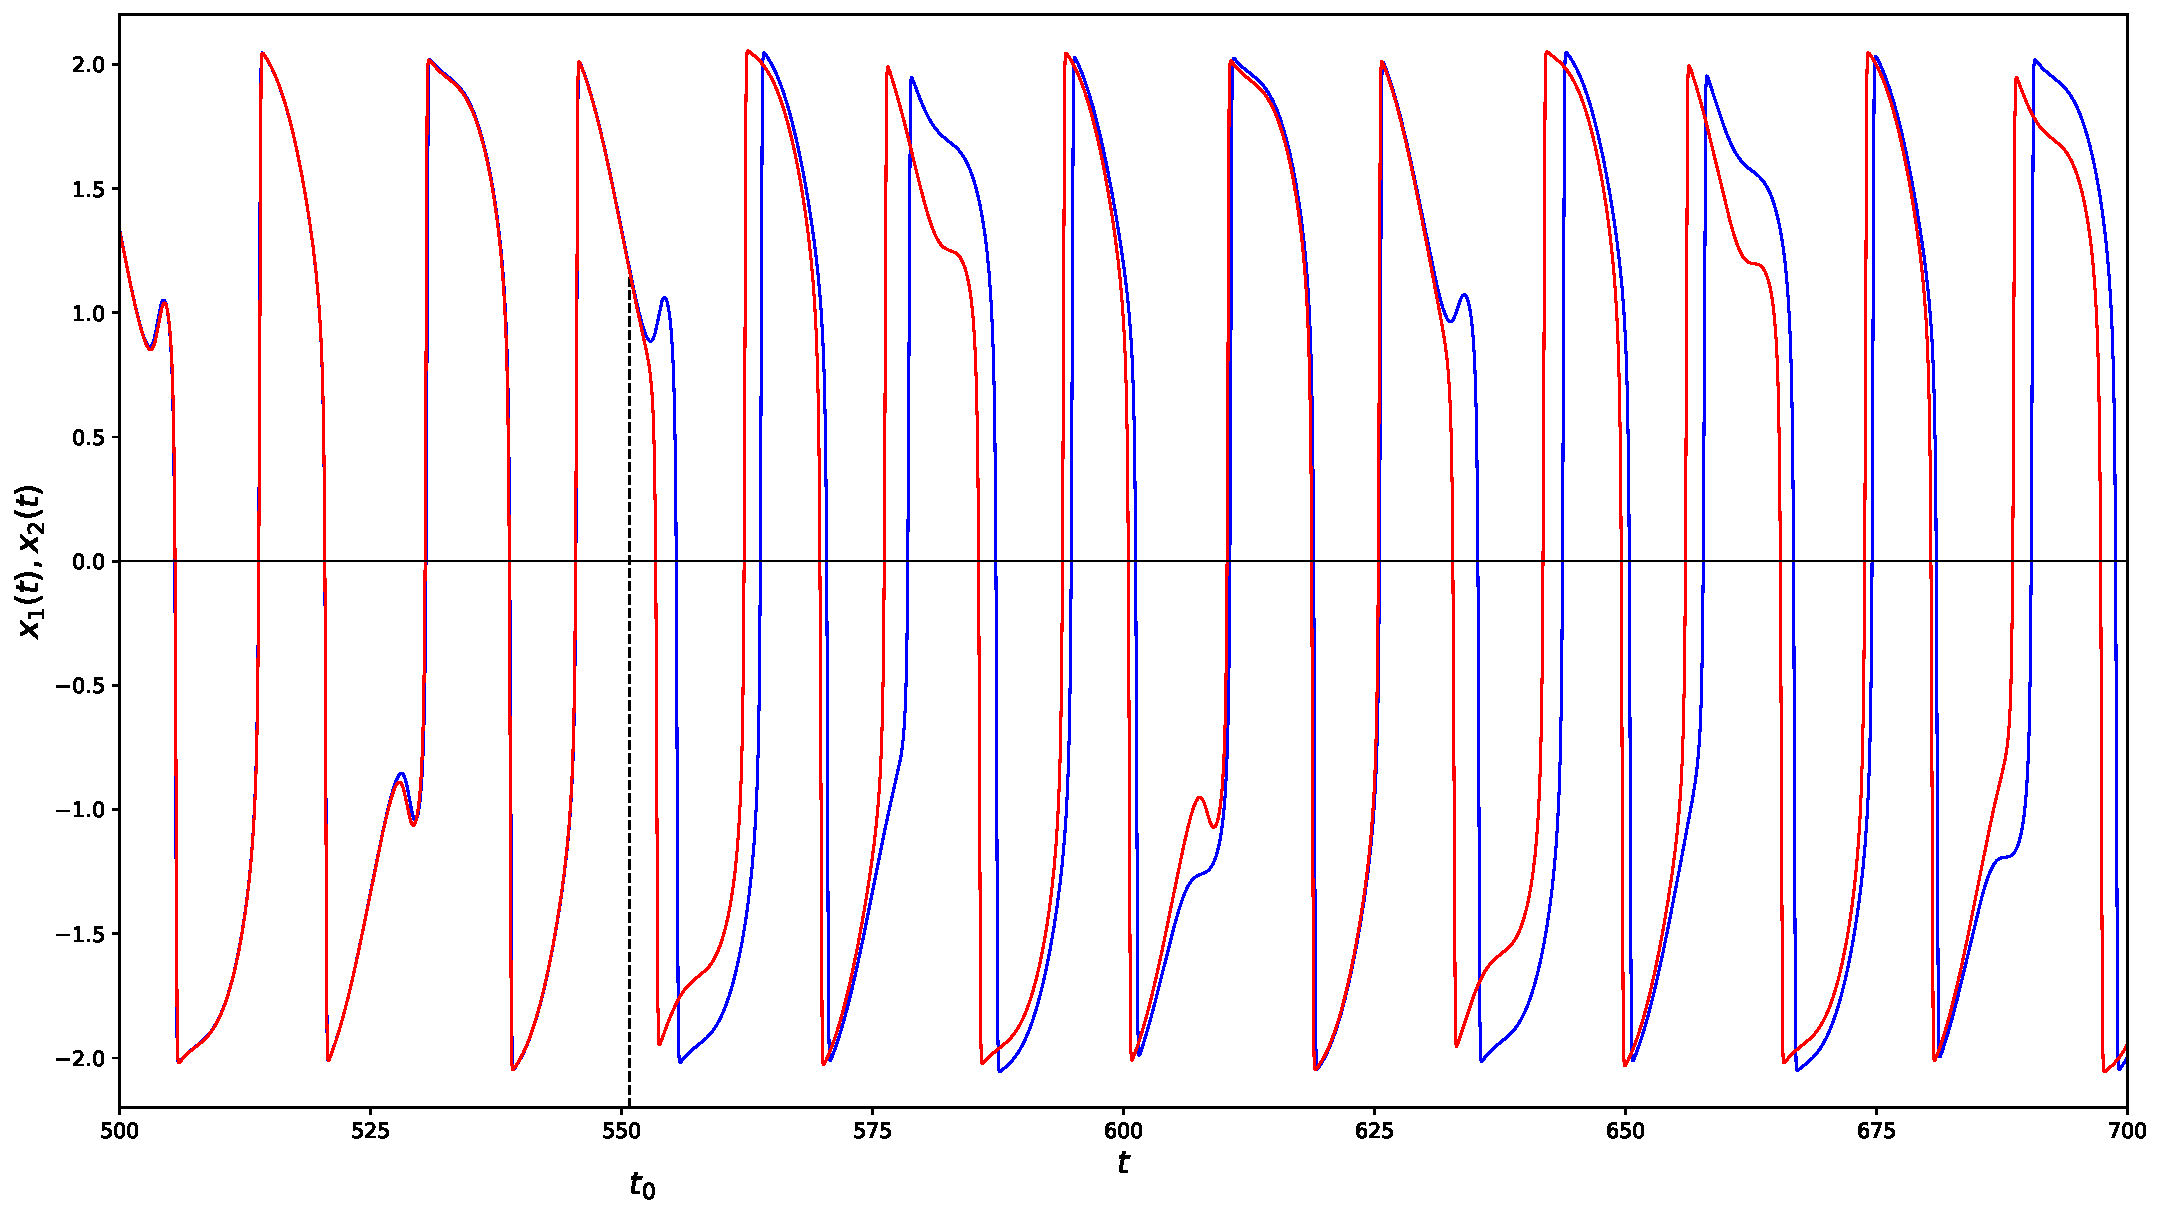
\includegraphics[width=\textwidth]{papers/vanderpol/figures/RK_schritt_delta_2e-3_2.pdf}
\caption{Verlauf der beiden mit der Runge Kutta Methode vierter Ordnung berechneten Lösungen $x_1$ und $x_2$ der Gl. \ref{vanderpol:equations:inhomogene_2} im Zeitbereich und Angabe des Divergenzpunktes $t_0$. Integrationsschritte: $h_1 = 0.007, \quad h_2 = 0.009$\label{vanderpol:figures:RK_schritt_2e-3}}
\end{figure}

\begin{figure}
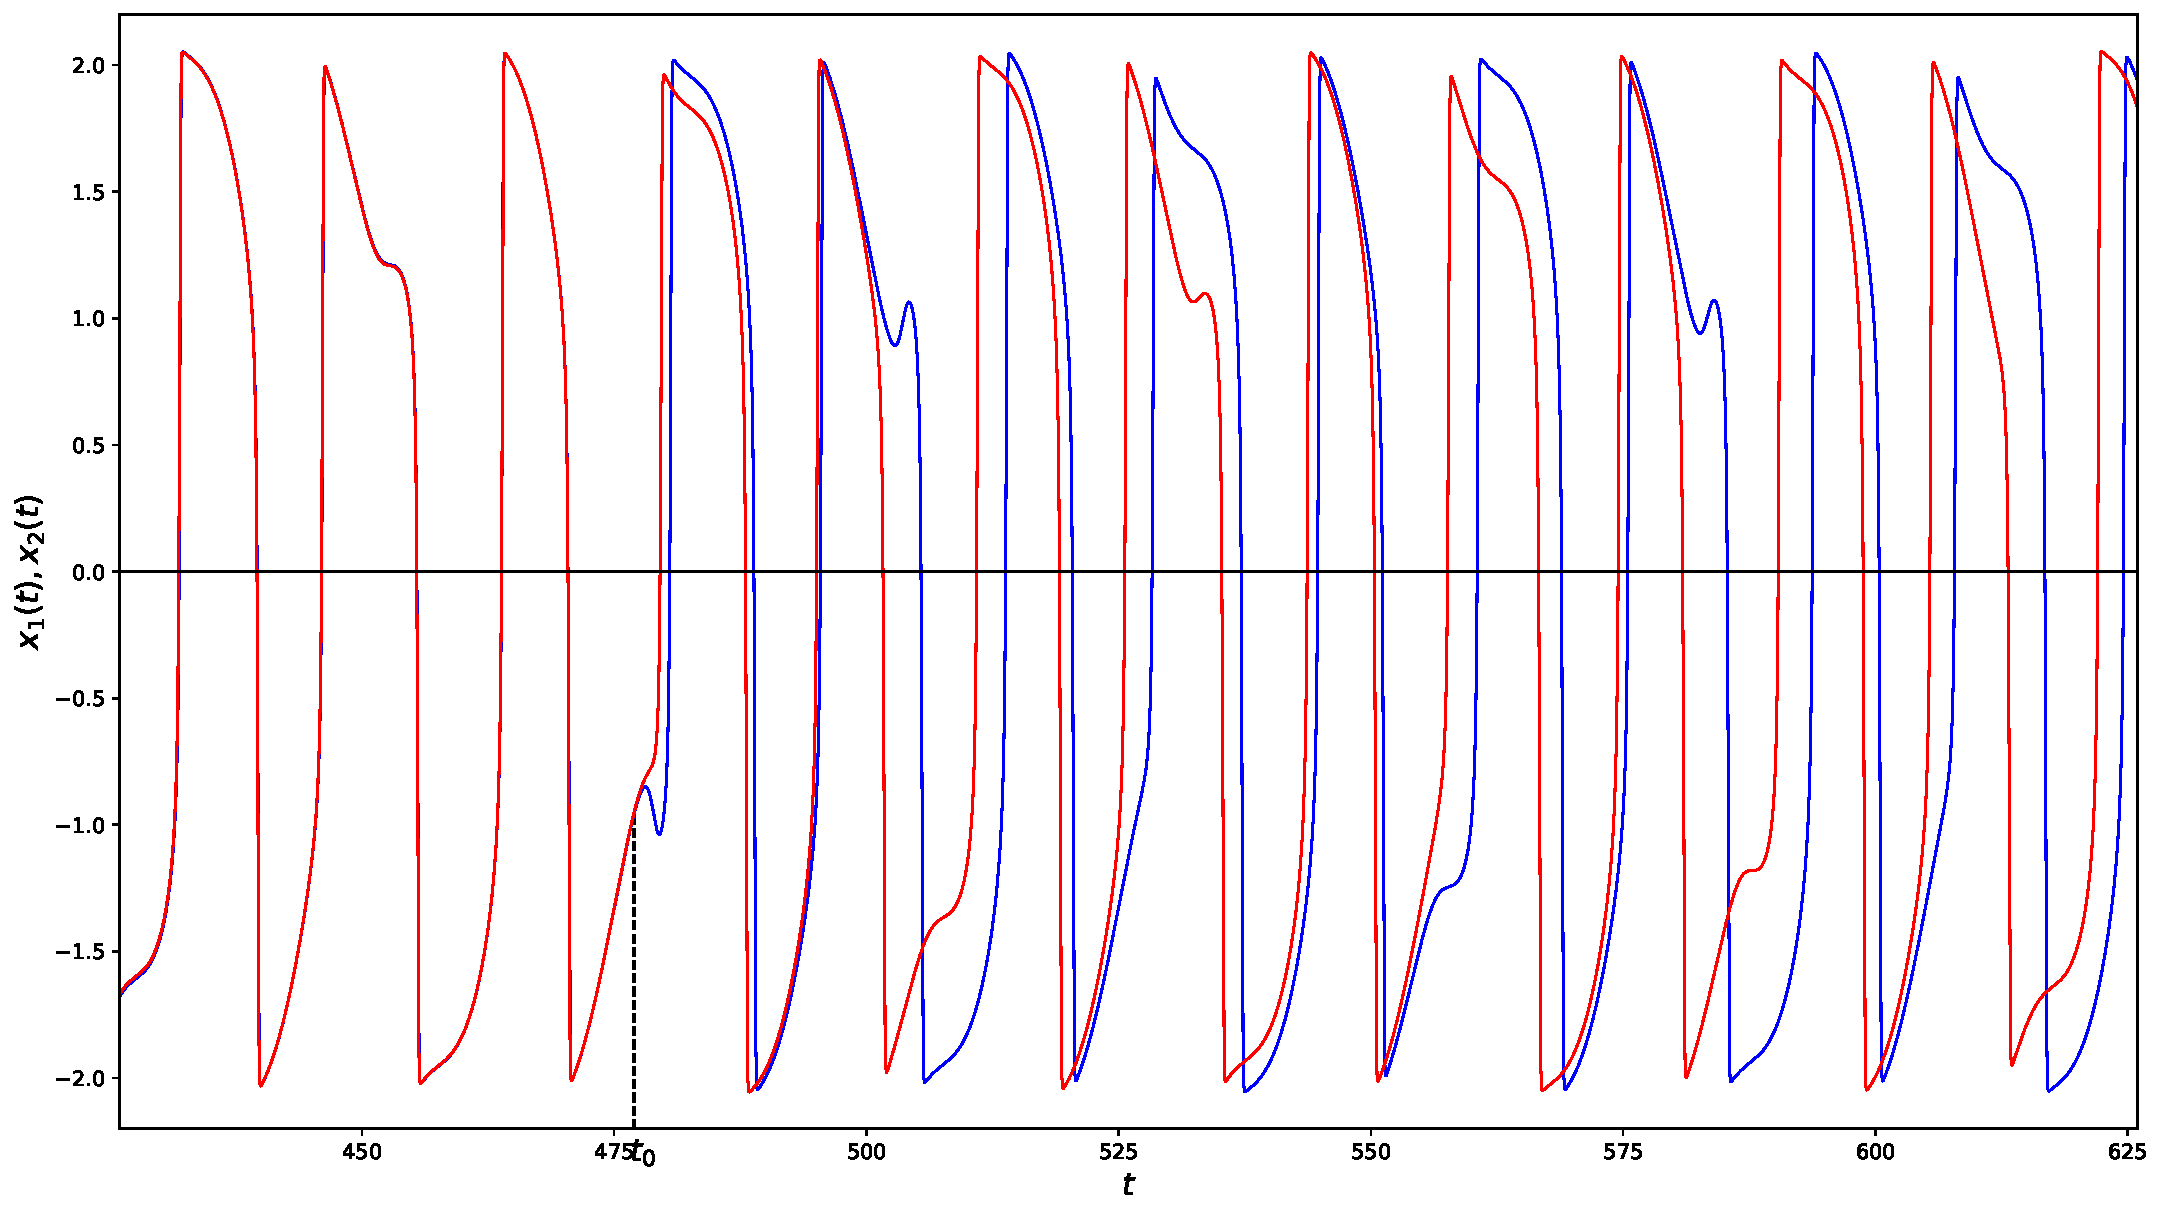
\includegraphics[width=\textwidth]{papers/vanderpol/figures/RK_schritt_delta_2e-3.pdf}
\caption{Verlauf der beiden mit der Runge Kutta Methode vierter Ordnung berechneten Lösungen $x_1$ und $x_2$ der Gl. \ref{vanderpol:equations:inhomogene_2} im Zeitbereich und Angabe des Divergenzpunktes $t_0$. Integrationsschritte: $h_1 = 0.005, \quad h_2 = 0.007$\label{vanderpol:figures:RK_schritt_2e-3_2}}
\end{figure}

